% =====================================================================
%  WACV 2026 — Applications Track — 8pp submission
%  "Viewpoint Invariance Is a Theorem, Not a Fit"
%  PRIMARY SOURCE for the WACV submission.
%  Compile:  pdflatex paper_wacv && pdflatex paper_wacv
%
%  DOUBLE-BLIND -- do not add to this file: \author content, an
%  acknowledgements or funding section, a repository URL, or a reference to
%  any non-anonymous version of this work. Comments travel with the .tex if
%  the source is ever shared, so keep them free of identifying material too.
% =====================================================================
\documentclass[10pt,twocolumn,letterpaper]{article}

\usepackage[review,applications]{wacv}   % review mode: line numbers + anonymized
\def\confName{WACV}
\def\confYear{2026}
\def\wacvPaperID{0000}  % <-- fill from CMT on submission

\usepackage{amsmath,amssymb,amsfonts,bm,mathtools}
\usepackage{graphicx}
\usepackage{booktabs}
\usepackage{multirow}
\usepackage{array}
\usepackage[breaklinks,colorlinks]{hyperref}
\usepackage[capitalize]{cleveref}

\newtheorem{proposition}{Proposition}

% Float and caption spacing. With 11 floats in an 8-page two-column body, the default separations
% cost several lines of column height in aggregate. Tightened here; typesetting only, no content or
% number changes, and still comfortably above the template's minimum legibility.
\setlength{\floatsep}{6pt plus 2pt minus 2pt}
\setlength{\textfloatsep}{8pt plus 2pt minus 2pt}
\setlength{\intextsep}{6pt plus 2pt minus 2pt}
\setlength{\abovecaptionskip}{4pt}
\setlength{\belowcaptionskip}{0pt}

\begin{document}

\title{Viewpoint Invariance Is a Theorem, Not a Fit:\\
An $SE(3)$-Equivariant Recurrence for Rehabilitation Exercise Assessment}
\author{}  % anonymized by [review] option
\maketitle

% =====================================================================
\begin{abstract}
A clinical screening instrument must return the same patient the same score from a different room. We
show that for skeleton-based rehabilitation assessment this per-prediction guarantee is available by
construction: an $SE(3)$-equivariant recurrent model whose read-out is invariant to camera viewpoint
as a \emph{theorem}, certified to the fp64 roundoff floor ($\sim\!10^{-16}$) over Haar-random
$SO(3)$ --- of which any camera relocation, including the $45^\circ$ NTU~RGB+D Cross-View
displacement, is one instance. On clean frontal
data no model separates from another --- ours, a point-cloud-transformer baseline, and a
hand-crafted-invariant GRU tie within a $0.33$~MAD nondeterminism floor --- so the benchmark's aggregate
metric is saturated and the decisive axis lies elsewhere: the augmented baseline
matches us in aggregate accuracy while still swinging an individual patient's score by up to $20.1$ MAD
(of $50$) under camera rotation, against our $9\times10^{-6}$. We then map the
accuracy--exactness--robustness--cost frontier and find that \emph{no model on it dominates}: the
point-cloud baseline is both the most accurate and the most node-robust, a hand-crafted-invariant
control is the cheapest and exactly invariant yet collapses under sensor-node failure, and a lighter
$E(n)$ encoder behind the identical invariant cut is measurably more brittle. Ours is the only point
that is exact \emph{by theorem} while clearing every stress up to three simultaneous node failures,
at $7.4\times$ fewer parameters. We
replicate the viewpoint and node-failure properties on a second corpus (REHAB24-6), and measure what
the theorem costs on the edge: an int8 activation-quantization cliff of only $0.05$ MAD --- $0.005$ of a
between-subject SD on this corpus, and one to two
orders of magnitude below MCID thresholds on comparable rehabilitation scales (\cref{sec:results})
--- and a causal streaming variant at $112$~fps (GPU, batch~1). We report our negative results --- a
null irregular-sampling regime and an unrewarded parity restoration --- with equal prominence.
\end{abstract}

% =====================================================================
\section{Introduction}\label{sec:intro}
Automated assessment of rehabilitation exercises from skeletons promises objective remote
monitoring~\cite{capecci2019kimore}. The dominant regime, however, trains and tests on clean frontal
recordings from one sensor and ranks models by a single aggregate error against a clinician's
score~\cite{karlov2024,abedi2023,kuang2026,pct2026}. It rewards capacity and penalizes nothing a
deployed device meets: a camera against a different wall, a tracking node that freezes, a dropped frame.

This paper argues that the \emph{regime}, not the architectures, is the problem. On clean frontal KIMORE
no architecture separates from another: our model, the point-cloud transformer, and a GRU on six
hand-crafted invariant features are statistically indistinguishable --- the benchmark's aggregate metric
is saturated. We can say so precisely because we first measured what a difference
must exceed to be one: training here is not bit-reproducible (nondeterministic cuDNN and scatter-add
kernels), and repeated fits of an \emph{identical} configuration differ by $\approx\!0.33$~MAD ---
larger than every clean-accuracy gap between the leading models. A single-run comparison on this
benchmark reports its own seed. Worse, auditing the reference transformer on the commonly used
single-exercise slice, optimistic epoch selection is worth $+1.2\pm0.4$~MAD ($18.6\%$ over three
seeds), and its honest number carries no reliable subject-level signal: the paired subject-cluster
bootstrap gives $\Delta=-0.44$ (per-seed $[-1.07,+0.20]$), clearing zero in only one of three seeds ---
the slice's limit, not the model's. We therefore
pool the five exercises, keep splits subject-disjoint, and gate every claim on clearing a per-exercise
mean-predictor floor --- a model that ignores its input has zero degradation and would win every
robustness plot. Pooled, every model we test clears it (\cref{tab:accuracy}).

With clean accuracy neutralized, the question becomes what a structural guarantee buys. We formulate
assessment as an \emph{invariant read-out of an equivariant representation}: a steerable
message-passing encoder produces per-joint features in $O(3)$ irreducible representations, an explicit
projection onto a generating set of invariants discharges the symmetry, and a recurrence consumes the
invariant code with the sensor's actual inter-arrival times (a capability KIMORE does not reward,
\cref{sec:results}; kept because it is free and demonstrably real off this corpus). Invariance of the score under any rigid
camera motion is then a \emph{theorem} (\cref{prop:invariance}), true for arbitrary weights, not a
behaviour induced by augmentation.

We contribute three things, none of them new invariance theory
(scalar contractions of Wigner-$D$-covariant features are invariant by
construction~\cite{geiger2022e3nn,thomas2018tfn,fuchs2020se3transformer}). An \emph{end-to-end
certification} protocol: eight numerical gates that survive the real steerable layers, the adaptive
solver and int8 quantization. An \emph{evaluation methodology} the field lacks: a mean-predictor floor
below which no gap is interpretable, and per-sequence degradation reported as a distribution rather
than a mean. And a \emph{deployment} analysis: a precision budget and a causal streaming read-out.
The distinction bites: a rotation-augmented baseline has a flat
\emph{aggregate} accuracy curve across azimuth --- by the field's metric it has solved viewpoint --- yet
its \emph{per-sequence} degradation averages $3.0$~MAD and reaches $20.1$ in the tail --- individual
scores swinging up to two fifths of the fifty-point scale as the camera moves, the errors merely
cancelling in the mean. Ours move by $9\times10^{-6}$; we report degradation and accuracy side by side
throughout.

The tie with the hand-crafted model leaves an obligation elegance cannot discharge: if a plain GRU on
named features is exactly as accurate \emph{and} as viewpoint-invariant, the steerable machinery is
unjustified. We discharge it against \emph{that} model specifically. When Kinect nodes freeze --- the
characteristic consumer-depth failure --- the hand-crafted model fails outright: a \emph{single} dead
joint drives it from $6.31$ to $9.78$~MAD, through the floor, because its features \emph{name} the
joints they depend on; the graph encoder pools learned messages and dilutes the failure across $25$
joints. That is one pairwise comparison, not an axis we own: the point-cloud baseline is more
node-robust than either of us, and our case rests on \emph{where} we sit on the
accuracy--exactness--robustness--cost frontier (\cref{tab:pareto}). We also treat
the guarantee as a \emph{systems} property: it survives to int8 (only activation-, not weight-rounding
perturbs it) and converts to strictly causal streaming at $8.9$~ms/frame. Finally we report the two places the structural story does not pay --- native consumption of irregular
arrivals, which a fixed grid beats at every drop level here, and a restored parity channel, principled
but unrewarded on healthy-form exercises.

\noindent\textbf{Contributions.}
(i) A protocol audit that establishes what the benchmark can measure --- an $18.6\%$ epoch-selection
inflation on the reference model, a $0.33$~MAD nondeterminism floor below which no accuracy gap is
interpretable, and a gated pooled protocol under which every model clears the floor. (ii) Exact viewpoint invariance, \emph{certified} by eight numerical gates (E1--E8)
over Haar-random $SO(3)$ rather than a single azimuth sweep, against a baseline that crosses
the floor by $45^\circ$. (iii) A Pareto characterisation of the
accuracy--exactness--robustness--cost frontier on which no model dominates: the baseline wins clean
accuracy \emph{and} node robustness, while ours is alone in being exact by theorem at $7.4\times$ fewer
parameters --- including, behind the identical invariant cut, evidence that lighter $E(n)$ equivariance
is more node-fail brittle. (iv) A second-corpus replication (REHAB24-6) of the viewpoint and node-failure
properties. (v) A co-designed deployment path: an int8 precision-budget audit and a causal streaming
read-out with an honest time-to-first-score. We also report two negative results, one of them derived.

% =====================================================================
\section{Related Work}\label{sec:related}
\textbf{Rehabilitation assessment and equivariant models.} KIMORE~\cite{capecci2019kimore} is the
standard benchmark; reported results span ST-GCN variants with contrastive
objectives~\cite{karlov2024}, cross-modal augmentation~\cite{abedi2023}, dual-stream graph
networks~\cite{kuang2026}, and point-cloud transformers~\cite{pct2026}, with
Rehab-Pile~\cite{rehabpile2026} (aggregating KIMORE, UI-PRMD~\cite{vakanski2018uiprmd} and IRDS) the closest antecedent of our protocol discipline. Evaluation is
uniformly in-distribution (same sensor, same placement, no simulated failure), and to our knowledge no
prior work reports a mean-predictor floor, without which a degradation curve cannot be interpreted.

Published numbers do not enter \cref{tab:accuracy}, because no protocol matches ours. Kuang et
al.~\cite{kuang2026} report MAD $0.10$--$0.16$ in the \emph{same} $0$--$50$ clinical-score units as our
subject-disjoint $6.3$--$6.7$, lower by a factor of $39$--$67$; their split is an explicit $8{:}1{:}1$
\emph{sample-level} stratified one. We recover those units from the published tables (supplement)
because the reference implementation standardises its targets and reading it wrong would move the
comparison by $8.5\times$. Karlov et al.~\cite{karlov2024} report Spearman $\rho$ rather than MAD, so we
report $\rho$ too: our pooled $\rho\!\approx\!0.6$ sits below the $0.74$--$0.965$ band the literature
spans, on a protocol whose mean-predictor null we also state. Abedi et al.~\cite{abedi2023} report only
a relative MAD reduction with no recoverable absolute baseline. Lacking their data and a
subject-disjoint rerun, we treat these as a different protocol, not an accuracy ceiling.

Group-equivariant networks impose symmetry as a constraint on the hypothesis class~\cite{cohen2016gconv};
the steerable family --- tensor-field networks~\cite{thomas2018tfn}, $SE(3)$-Transformers~\cite{fuchs2020se3transformer},
\texttt{e3nn}~\cite{geiger2022e3nn} --- guarantees equivariance for arbitrary weights, while lighter
constructions reach $E(n)$-equivariance without spherical harmonics~\cite{satorras2021egnn} or via
vector neurons~\cite{deng2021vectorneurons}. We build on~\cite{geiger2022e3nn}, but the claim is
\emph{not} about steerable machinery: a GRU on hand-crafted invariants attains the same accuracy and
viewpoint guarantee at a third of the parameters, and we isolate the one axis on which they differ
(\cref{tab:nodefail}).

\textbf{Invariance by canonicalization, augmentation, and corruption robustness.} A non-equivariant
backbone can be made invariant by canonicalization or frame averaging~\cite{puny2022frameaveraging},
exact only in so far as the frame estimate is --- a point estimate whose \emph{conditioning} degrades
near covariance degeneracy, which we measure directly (\cref{sec:results}); our cut estimates no frame,
being an explicit projection exact for arbitrary weights (\cref{prop:invariance}). Training-time augmentation flattens
\emph{aggregate} error but makes per-prediction errors cancel, not vanish --- expressible only if
degradation is reported per sequence. For irregular sampling, the standard alternatives are
resampling or continuous-time models~\cite{chen2018neuralode,rubanova2019odernn,kidger2020neuralcde,che2018grud};
we implement the Neural CDE variant (adaptive Dormand--Prince solver~\cite{dormand1980prince}) as a certified \emph{control} that fails the floor. Occlusion and
tracking failure are usually met with masking or attention~\cite{yan2018stgcn}; we adopt the failure
literally, as the discriminating experiment between two otherwise-indistinguishable models.

\begin{figure*}[t]\centering
  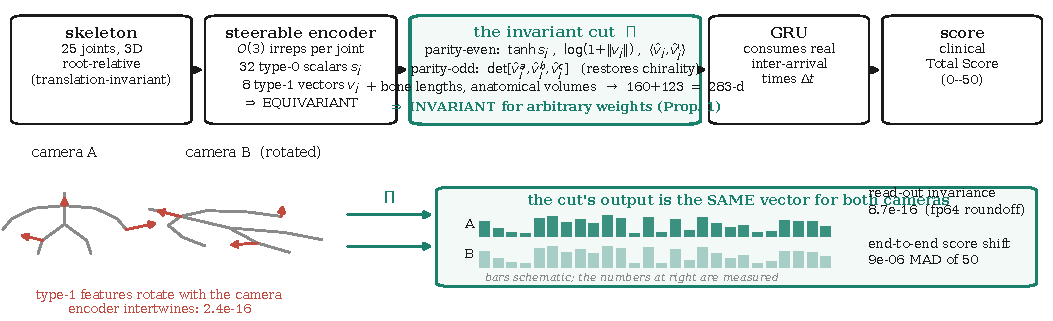
\includegraphics[width=\textwidth]{fig_method}
  \caption{\textbf{The invariant cut is the method.} Top: the pipeline. Bottom: the same pose at two
  camera poses --- the encoder's type-1 features rotate (equivariance), the cut's output does not
  (invariance, Prop.~\ref{prop:invariance}). Bar heights are schematic; the annotated quantities are
  measured (\texttt{certify\_egru.json}, \texttt{final\_tables.json}).}
  \label{fig:method}
\end{figure*}

% =====================================================================
\section{Method}\label{sec:method}
A steerable encoder on the skeleton graph carries per-joint latents in $O(3)$ irreps ($n_0$ type-$0$
scalars $s_j$, $n_1$ type-$1$ vectors $v_j$); feeding \emph{root-relative} coordinates makes
translation invariance automatic. The encoder is \emph{equivariant}; the score must be \emph{invariant}.

\textbf{The invariant cut.} The transition is an explicit projection $\Pi$ onto a generating set of
invariants. The parity-even generators (scalars, vector norms, pairwise cosines) are complete for the
full $O(3)$ --- each is fixed by a reflection --- so a cut built from them is blind to \emph{trajectory
handedness} (a clockwise and anticlockwise limb circle share every bone length, distance and speed). We
complete it with parity-odd pseudo-scalar triple products over unit vectors:
\begin{align}
\pi_j^{\mathrm{even}} &= \Big[\tanh s_j \,\|\, \log(1{+}\|v_j^{c}\|)_c \,\|\,
  \langle\hat v_j^{c},\hat v_j^{c'}\rangle_{c<c'}\Big] \label{eq:cut-even}\\
\pi_j^{\mathrm{odd}} &= \Big[\det[\hat v_j^{a},\hat v_j^{b},\hat v_j^{c}]_{a<b<c}\Big]
  \label{eq:cut-odd}\\
\pi_j &= \big[\pi_j^{\mathrm{even}} \,\|\, \pi_j^{\mathrm{odd}}\big] \label{eq:cut}
\end{align}
with $\hat v=v/\|v\|$, pooled over joints by mean$\oplus$max and concatenated with invariant bone
lengths and a fixed set of anatomical signed volumes $\chi_\tau$ (index-preserved, unpooled):
\begin{equation}\label{eq:pi}
\Pi(h,\tilde{\bm{x}})=\big[\,\mathrm{mean}_j\pi_j \,\|\, \max_j\pi_j \,\|\, (d_{ij})_{\mathcal{E}} \,\|\, (\chi_\tau)_{\mathcal{T}}\,\big].
\end{equation}
At the deployed widths ($n_0{=}32$, $n_1{=}8$) the parity-even subtotal is $160$-d and the parity-odd
completion adds $123$-d ($283$-d total; full specification in the supplement). A liveness gate zeroes
any generator touching a failed joint, which makes the dead-node \emph{invariance} certified by E1--E8
exact under a known failure mask; the degradation reported in \cref{tab:nodefail} instead uses the
deployed gate-\emph{off} model with no failure signal supplied, so the graceful fall-off measured there
is message-passing dilution alone, not the gate.

\begin{proposition}[$SO(3)$-invariance of the read-out]\label{prop:invariance}
For an encoder that intertwines with the Wigner-$D$ action on its latents, $\Pi$ of \cref{eq:cut}--\eqref{eq:pi}
is invariant under $SO(3)$ for \emph{arbitrary} weights; the predicted score is therefore invariant to
any rigid motion of the camera. (Proof in the supplement.)
\end{proposition}

\textbf{Certificate.} We audit the read-out with eight numerical gates (\cref{tab:certificate}), all
passed, each independently re-runnable and refutable (see Code availability): representation orthogonality
$\le10^{-12}$; violation at the fp64 roundoff floor ($\sim\!10^{-16}$) with a \emph{flat} log--log
slope in rotation angle ($|\text{slope}|<0.5$, against $\approx\!1$ for a genuine modelling error) and
an fp32/fp64 violation ratio $>\!10^{8}$ (excluding a small modelling violation masquerading as noise);
translation and read-out invariance both $\sim\!10^{-16}$ (fp64) after the parity-odd channels are admitted. The guarantee is over Haar-random
proper rotations of the \emph{full} $SO(3)$, of which a camera azimuth or a cross-view displacement is
one instance. A continuous-time (Neural CDE) variant, certified to the same standard, \emph{fails} the
mean-predictor floor and is reported only as a control (supplement).

\begin{table}[t]\centering\small
\setlength{\tabcolsep}{4pt}
\caption{\textbf{The viewpoint guarantee is falsifiable.} Eight numerical gates on the deployed
read-out: E1--E5 that the invariance is \emph{present}, E6--E8 that it is the \emph{intended} one
(chirality live, laterality preserved). Roundoff-floor quantities are regime-stable, not
bit-reproducible (representative fp64 run); E6--E7 are \emph{modelling} quantities, not roundoff,
reported for seed~0 of \texttt{certify\_egru.json}. Parity/laterality gates report the
even\,/\,chiral cut.}
\label{tab:certificate}
\begin{tabular}{clc}
\toprule
Gate & Criterion & Result \\
\midrule
E1 & rep.\ orthogonality $\|\rho^{\!\top}\!\rho{-}I\|_F$ & $\le10^{-12}$ \checkmark \\
E2 & motion-channel invariance & verified \checkmark \\
E3 & rotation-sweep violation\,/\,slope & $\sim\!10^{-16}$, $|{\cdot}|{<}0.5$ \checkmark \\
E4 & fp32/fp64 violation ratio $r$ & $>\!10^{8}$ \checkmark \\
E5 & translation invariance & $\sim\!10^{-16}$ \checkmark \\
E6 & parity (even\,/\,chiral) & $0$ / $4.4\!\times\!10^{-2}$ \\
E7 & laterality (even\,/\,chiral) & $6.9$ / $5.6\!\times\!10^{-2}$ \\
E8 & full-$SO(3)$, parity-odd active & $\sim\!10^{-16}$ \checkmark \\
\bottomrule
\end{tabular}
\end{table}

% =====================================================================
\section{Results}\label{sec:results}
All experiments are pooled, subject-disjoint, over 3 seeds, except the TCN, ST-GCN and Ridge
viewpoint curves of \cref{fig:viewpoint}, which are 5-fold cross-validated at a single seed.
\emph{Protocol audit}
(\cref{tab:protocol3seed}): we audit the point-cloud transformer baseline on the single-exercise slice
most commonly reported. Honest epoch selection removes an $18.6\%$ inflation (3 seeds) and leaves that
model with no robust separation from a mean predictor --- the paired subject-cluster bootstrap gives
$\Delta=-0.44$ and clears zero in only $1/3$ seeds. This is not
subject leakage (each subject contributes one recording on that slice, so a random split is already
subject-disjoint); the slice simply carries no robust subject-level signal, which is why we pool the
five exercises and gate every experiment on a per-exercise mean-predictor floor. Pooled, \emph{every}
model here clears that floor (\cref{tab:accuracy}).

\begin{table}[t]\centering\small
\setlength{\tabcolsep}{5pt}
\caption{Protocol audit of the \emph{point-cloud transformer baseline}, single-exercise slice (KIMORE
Ex.~1; subject-disjoint 5-fold; 3 seeds). \emph{Honest} selects the epoch on a held-out validation fold;
\emph{inflated} takes the per-epoch test minimum (the reference protocol). $\Delta$ is the paired
subject-cluster bootstrap $\text{MAD}(\text{honest})-\text{MAD}(\text{floor})$; an interval below $0$
means the model beats the mean predictor. The signal here is \emph{seed-fragile}, clearing zero in only
$1/3$ seeds; pooling fixes this, for this model and every other (\cref{tab:accuracy}).}
\label{tab:protocol3seed}
\resizebox{\columnwidth}{!}{%
\begin{tabular}{lccc}
\toprule
Seed & Honest / Inflated & Selection bias & $\Delta$ vs.\ floor \ (95\% CI) \\
\midrule
0    & $6.90 / 5.45$ & $+1.44\ (20.9\%)$ & $+0.20\ [-0.59,+1.03]$ \\
1    & $6.53 / 5.00$ & $+1.54\ (23.5\%)$ & $-0.46\ [-1.60,+0.72]$ \\
2    & $5.84 / 5.17$ & $+0.67\ (11.4\%)$ & $\mathbf{-1.07\ [-1.98,-0.15]}$ \\
\midrule
mean & $6.42{\pm}0.44 / 5.21{\pm}0.19$ & $+1.22\ (18.6\%)$ & $-0.44$ \\
\bottomrule
\end{tabular}}
\end{table}

\textbf{The clean-accuracy metric is saturated.} EGRU ($6.73\pm0.30$), a GRU on hand-crafted invariants
(InvariantGRU, $6.31\pm0.16$), and the point-cloud transformer (PCT, $6.47\pm0.20$) are mutually
indistinguishable: every gap is inside the $0.33$~MAD seed floor (\cref{tab:accuracy}). This is a
statement about the models \emph{relative to each other}, not about whether any of them carries real
subject-level signal: unlike the fragile single-exercise slice (\cref{tab:protocol3seed}, clears zero in
only $1/3$ seeds), the pooled bootstrap $\Delta$ vs.\ floor is entirely below $0$ for all three
--- PCT $-1.87\,[-2.72,-1.06]$, InvariantGRU $-2.03\,[-2.88,-1.23]$, EGRU $-1.60\,[-2.37,-0.88]$
--- so the tie is a tie among models that each genuinely beat the mean predictor, not three models
indistinguishable from noise. The tie survives the metric change: Spearman $\rho$ separates the same
models by at most $0.05$ (\cref{tab:accuracy}), so saturation is a property of the benchmark, not of
the error measure chosen to report it. $\rho$ also needs its null stated --- the mean predictor scores
pooled $\rho=0.17$ while ignoring its input entirely, and exactly $0$ once the between-exercise
score differences it exploits are removed. A benchmark on
which three architectures of vastly different inductive bias cannot be told apart is not measuring
architecture --- which is the premise for evaluating on an axis that can. Restoring
chirality ($O(3)\!\to\!SO(3)$) costs $+0.11$~MAD for EGRU --- inside the floor --- for $16.7\%$ more
parameters and the removal of a silent handedness assumption; we adopt the chiral model on that basis,
not an accuracy one. The chiral read-out's wider seed spread ($\pm0.30$ vs $\pm0.08$ for the parity-even
model) reflects the added parity-odd capacity, not instability --- every seed stays inside the floor.

One asymmetry against the baseline is worth closing: EGRU sees a one-hot exercise id and the floor is
per-exercise, so pooled PCT alone was scored blind to the exercise. Re-training it with identical
conditioning (3 seeds, both arms) changes nothing: clean $6.59\pm0.07$ vs.\ $6.47\pm0.20$, augmented
$7.42\pm0.22$ vs.\ $7.47\pm0.23$ --- inside the floor and opposite in sign --- and the per-sequence
swing is if anything \emph{larger} ($21.43$ vs.\ $20.12$~MAD worst sequence). Viewpoint fragility is not
an artefact of withholding exercise identity; we report the unconditioned arm throughout.

\begin{table}[t]\centering\small
\setlength{\tabcolsep}{4pt}
\caption{Clean-data accuracy (pooled, subject-disjoint, mean$\pm$std over 3 seeds). The $0.33$~MAD floor
is the \emph{fixed-configuration} one; the wider seed-to-seed spread ($0.48$) is in the supplement.
$\Delta$ vs.\ floor is the paired subject-cluster bootstrap of \cref{tab:protocol3seed} ($n{=}77$
subjects, checkpoints re-evaluated without retraining; \texttt{pooled\_bootstrap\_eval.py}). Spearman
$\rho$ is computed per seed on that seed's complete out-of-fold vector, pooled over exercises and again
within each exercise.}
\label{tab:accuracy}
\resizebox{\columnwidth}{!}{%
\begin{tabular}{llccccc}
\toprule
& & & & \multicolumn{2}{c}{Spearman $\rho$ $\uparrow$} & \\
\cmidrule(lr){5-6}
Model & Group & MAD $\downarrow$ & Params & pooled & within-ex. & $\Delta$ vs.\ floor (95\% CI) \\
\midrule
PCT (baseline)              & ---     & $\mathbf{6.47\pm0.20}$ & $4.91$M & $0.60\pm0.02$ & $0.55\pm0.02$ & $-1.87\ [-2.72,-1.06]$ \\
PCT $+$ rotation aug.       & ---     & $7.47\pm0.23$ & $4.91$M & ---           & ---           & --- \\
InvariantGRU (hand-crafted) & $SO(3)$ & $\mathbf{6.31\pm0.16}$ & $0.21$M & $0.59\pm0.01$ & $\mathbf{0.56\pm0.01}$ & $-2.03\ [-2.89,-1.23]$ \\
\textbf{EGRU (ours)}        & $SO(3)$ & $\mathbf{6.73\pm0.30}$ & $0.66$M & $0.56\pm0.04$ & $0.52\pm0.04$ & $-1.60\ [-2.37,-0.88]$ \\
\midrule
Mean-predictor floor        & ---     & $8.31\pm0.05$ & --- & $0.17\pm0.01$ & $-0.07\pm0.02$ & --- \\
\bottomrule
\end{tabular}}
\end{table}

\textbf{Viewpoint invariance is a theorem, not a fit} (\cref{fig:viewpoint}). Across test-time camera
azimuth the certified-invariant models are flat to machine precision (EGRU mean
$9\times10^{-6}$~MAD, worst single sequence $3\times10^{-4}$; InvariantGRU exactly $0$; hand-crafted invariant features Ridge at the fp64
roundoff floor, $10^{-14}$ --- both invariant by construction, so these two curves are a
positive control, not independent evidence),
while all non-equivariant baselines degrade catastrophically: PCT crosses the mean-predictor floor between
$30^\circ$ and $45^\circ$ (mean per-sequence shift $9.33$~MAD at its worst angle, worst sequence
$33.96$ of fifty); TCN $13.17$~MAD; ST-GCN $9.18$~MAD. The pattern holds across three
independently-designed non-equivariant architectures (temporal-conv, graph-conv, attention):
viewpoint fragility is generic to non-equivariance, not PCT-specific. Rotation augmentation flattens PCT's aggregate curve but leaves a \emph{per-sequence}
score shift averaging $3.01$~MAD --- and the average is the wrong statistic for a clinical claim: the
$95$th percentile is $8.65$~MAD and the worst single held-out sequence moves $20.12$ (a global maximum
over all $380$ held-out sequences $\times\,3$ seeds; the fold-averaged max would read a flattering
$12.81$), two fifths of the scale and $2.01$ between-subject SD, purely because the camera moved. This is the difference between a guarantee and a fit. It is not
an undertraining artefact: at $3\times$ and $9\times$ the epoch budget the shift stays flat
($3.01$/$3.27$/$2.94$~MAD mean at $60$/$180$/$540$ epochs, worst $20.1$/$21.4$/$19.9$), so it is what augmentation
converges to --- though we varied the budget, not augmentation strength, and a differently tuned
schedule may narrow the gap.

\textbf{On NTU the guarantee is measured, not inherited.} A Haar-random $SO(3)$ rotation of all
$18{,}674$ Cross-View test clips changes \emph{not one} prediction (agreement $100.00\%$, Top-1
$82.95\%$ unchanged; drift $2.3\times10^{-13}$ in fp64, $5.7\times10^{9}$ below fp32 --- roundoff),
where ST-GCN agrees on $91.89\%$, loses $3.03$ points, with a drift precision cannot move (ratio
$1.0008$): structural, not numerical. Both are within-model. But a rotated skeleton is not a
relocated camera: NTU films each performance at three cameras \emph{at once}, and on those
$18{,}674$ triples --- three skeleton \emph{estimates} of one event --- our agreement falls to
$73.03\%$ against ST-GCN's $73.86\%$: a small but resolvable deficit (paired exact binomial,
$5{,}394$ discordant triples, $p{=}0.037$), still confounded by the protocol caveat below. The
theorem removes a viewpoint change's geometry exactly and none of the tracker noise a relocation
adds; reporting the rotation alone would overstate it.
NTU otherwise contributes generalisation: trained \emph{without} rotation augmentation on cameras
$2$--$3$ and tested on camera $1$, the encoder reaches $82.98\%$ Top-1 ($T{=}100$, single-clip, one
seed) --- also why it sits below the $\sim\!88\%$ for this split. We give no ST-GCN accuracy control:
our runs differ in sampling, view-normalisation and optimiser, so the pair would not compare.

\begin{figure}[t]\centering
  
\includegraphics[width=\linewidth]{fig_viewpoint}
  \caption{MAD vs.\ camera azimuth. Certified-invariant models (EGRU, InvariantGRU, hand-crafted Ridge)
  are flat by theorem; all non-equivariant baselines (PCT, TCN, ST-GCN) degrade $9$--$13$~MAD at
  extreme angles --- viewpoint fragility is generic to non-equivariance. Augmentation flattens PCT's
  aggregate but not its per-sequence swing (mean $3.01$~MAD, worst sequence $20.12$). Azimuth here is
  a rigid rotation of the ground-truth Kinect skeletons; it isolates the geometric effect of viewpoint
  and does not model per-view tracker degradation, which we measure separately on a physically
  relocated camera (supplement).}
  \label{fig:viewpoint}
\end{figure}

\textbf{Clinical interpretation of the MAD scale.} No inter-/intra-rater reliability coefficient (ICC,
$\kappa$) is reported for KIMORE's clinical Total Score~\cite{capecci2019kimore} or for REHAB24-6's; a
targeted search, including direct attempts to retrieve the Capecci et al.\ full text (both the publisher
record and the indexed copy returned access-blocked to automated retrieval), could not surface one, and
we do not fabricate one --- we flag its absence as this paper's clearest open measurement gap. As
external context, \emph{movement-quality rating} --- the construct KIMORE's clinicians perform, not a
functional-recovery outcome --- shows moderate-to-good inter-rater agreement (Cutting Movement
Assessment Score ICC $0.58$--$0.91$; cross-diagnostic Movement Quality Score $0.93$): a defensible band
on what a KIMORE-specific coefficient would show, not a substitute for one. As a magnitude-of-change
cross-check from a different construct and scale, minimal clinically important differences (MCIDs) on
comparable $0$--$66$/$0$--$100$-point motor-\emph{recovery} scales sit in the low single digits to low
teens (Fugl-Meyer upper-extremity $4$--$12.4$, lower-extremity $6$, Stroke Rehabilitation Assessment of
Movement $1.9$--$4.8$ per subscale), putting the augmented baseline's per-sequence swing (mean $3.01$,
worst sequence $20.12$, of $50$) in the same order of magnitude as an established change-significance
threshold on cognate instruments --- at the tail, above it --- and our own score shifts under rotation
($9\times10^{-6}$), int8 and streaming ($0.05$ and lower, \cref{sec:edge}) orders of magnitude below it.
A camera relocation that moves a patient's score by more than an MCID is a measurement the instrument
cannot be trusted to make; that is the practical content of the guarantee.
The sharper, in-dataset question --- does a $3.01$-point swing cross KIMORE's clinical
bands? --- has no answer: those bands do not exist, the five groups being recruitment categories, with
a control scoring below a patient on every exercise (Es5: Expert $25.0$, Parkinson $50.0$). Measured
against the score's actual resolution, the mean swing is $0.30$ between-subject SD and the worst
sequence $2.01$ SD, and it exceeds the gap separating $20.2\%$ of subject pairs, $83.0\%$ at the tail
--- pairs a camera can reorder (supplement). The MCID band then reads as corroboration from adjacent
instruments, not as a KIMORE-specific threshold and not as the load-bearing claim.

\textbf{Does the guarantee cost robustness? Sensor-node failure} (\cref{tab:nodefail}). This is a tax
check, not a selling point. Freezing $k$ tracking nodes at their first-frame pose, the hand-crafted arm
collapses through the floor at a \emph{single} dead joint ($6.31\!\to\!9.78$) because its features name
their joints; EGRU pools learned graph messages and loses $+3.76$~MAD over $8$ dead joints.
\textbf{PCT wins this axis outright} ($+2.27$): it leads on KIMORE and, on REHAB24-6, overtakes us
between $k{=}2$ and $k{=}4$ and finishes $0.021$~AUROC ahead at $k{=}8$ (supplement). Node robustness is
not a property of equivariance and we do not claim it. The table supports something narrower: the
guarantee is not paid for with a robustness collapse ($k{=}8$ crosses the floor for every model, EGRU
included). Both models see identically corrupted joints with no imputation, and we measured the
fairness objection rather than assuming it: an \emph{oracle} liveness mask (told which joint died, no
retraining) closes only $\sim\!25\%$ of the gap to EGRU ($+12.05\!\to\!+10.02$~MAD; \cref{tab:nodefail},
right) --- the graph encoder needs no such signal and loses far less, so the gap is architectural, not
a missing-information artifact. The mechanism is invariant to the failure model (five operators incl.\
lag/burst/axis/lateral; supplement).

\begin{table}[t]\centering\small
\setlength{\tabcolsep}{4pt}
\caption{Sensor-node failure: MAD as $k$ nodes freeze (mean over 3 seeds $\times$ 5 folds; identical
hash-locked inputs; no retraining). \underline{Underline}: past the floor ($8.31$). ``+oracle'':
InvariantGRU given an oracle liveness mask (same checkpoint; features touching the dead joint zeroed
at inference) --- the measured fairness control.}
\label{tab:nodefail}
\resizebox{\columnwidth}{!}{%
\begin{tabular}{rcccc}
\toprule
Dead nodes $k$ & EGRU (ours) & InvariantGRU & \;+oracle & PCT \\
\midrule
$1$ & $7.10$ & \underline{$9.78$}  & \underline{$9.39$}  & $6.76$ \\
$4$ & \underline{$8.41$} & \underline{$15.96$} & \underline{$15.25$} & $7.51$ \\
$8$ & \underline{$10.50$} & \underline{$18.37$} & \underline{$16.33$} & \underline{$8.73$} \\
\midrule
MAD lost & $+3.76$ & $+12.05$ & $+10.02$ & $\mathbf{+2.27}$ \\
\bottomrule
\end{tabular}}
\end{table}

\textbf{The mechanism is not an artifact of the freeze model.} Under four further operators ---
stuck-at-lag, bursts, single-axis depth noise, left-limb-only --- the ordering is invariant: the
hand-crafted arm degrades most and the graph-pooled encoder least among the two exact-invariance
models (\cref{tab:nodefail_modes}). \emph{Persistent} faults (freeze, lag) hurt naming features far
more ($+12.05$, $+8.88$) than \emph{transient} ones (burst $+2.83$, axis $+1.93$) --- a length-masked
temporal mean dilutes an intermittent spike but not a permanently corrupted coordinate --- and
unilateral failure does not break the parity channels (InvariantGRU $+8.73$, EGRU $+3.43$).

\begin{table}[t]\centering\scriptsize
\setlength{\tabcolsep}{3pt}
\caption{Node failure under five operators (chiral models, 3 seeds $\times$ 5 folds, hash-locked).
Each cell: MAD at $k{=}1$ / $k{=}8$ and total lost. The freeze/random row reproduces
\cref{tab:nodefail}.}
\label{tab:nodefail_modes}
\resizebox{\columnwidth}{!}{%
\begin{tabular}{lccc}
\toprule
Failure operator & EGRU (ours) & InvariantGRU & PCT \\
\midrule
freeze (random)    & $7.10/10.50\,({+}3.76)$ & $9.78/18.37\,({+}12.05)$ & $6.76/8.73\,({+}2.27)$ \\
freeze (left-only) & $7.11/10.16\,({+}3.43)$ & $10.81/15.04\,({+}8.73)$ & $6.83/9.62\,({+}3.15)$ \\
stuck-at-lag       & $6.82/7.76\,({+}1.03)$  & $9.02/15.19\,({+}8.88)$  & $6.60/7.11\,({+}0.64)$ \\
sporadic burst     & $6.74/6.78\,({+}0.05)$  & $6.69/9.14\,({+}2.83)$   & $6.47/6.45\,({-}0.02)$ \\
axis/depth noise   & $6.77/7.20\,({+}0.47)$  & $6.70/8.24\,({+}1.93)$   & $6.48/6.50\,({+}0.03)$ \\
\bottomrule
\end{tabular}}
\end{table}

\textbf{The whole thesis in one grid} (\cref{tab:pareto}). \emph{No model wins all five columns}, and
that --- not any single stress --- is the claim. PCT is both the most accurate clean model ($6.47$) and
the most node-robust ($7.10$); InvariantGRU is the cheapest at exactly zero degradation yet collapses at
two dead nodes ($11.64$); and three models clear every stress --- ours, Canon-PCA$+$PCT, and
rotation-augmented PCT --- so we are not the only survivor. Among those three, ours alone runs at
$0.66$M rather than $4.91$M parameters and alone rests on a theorem rather than an estimated frame or
an augmentation tolerance. What separates the survivors is the last column (\cref{fig:guarantee}a):
all flat in aggregate, but the augmented baseline's mean per-sequence degradation is $3.01$~MAD (worst
sequence $20.12$) against our $9\times10^{-6}$ ($3.0\times10^{-4}$ worst), at $7.4\times$ more
parameters. This is the only categorical difference rather than a trade: $3.01$ is a tolerance that
happens to be small on this data and has a $20$~MAD tail; $9\times10^{-6}$ is roundoff around a value
the theorem fixes at zero. Every other column is an axis we may lose, and on node failure we do.
Behind the \emph{identical} cut, a lighter $E(n)$ (EGNN) encoder ties clean accuracy and viewpoint
(exact by construction) but is more node-fail brittle: tuned across depth, width, and coordinate-clamp
over three seeds it loses $+6.4\pm1.3$~MAD over eight dead joints (vs.\ $+3.76$) and crosses the floor
already at two ($8.44$ vs.\ $7.55$) --- the steerable encoder is the more robust equivariant option.

\begin{table}[t]\centering\small
\setlength{\tabcolsep}{4pt}
\caption{Does each model clear the floor ($8.31$~MAD) under each stress? The node column is $k{=}2$;
the full sweep is \cref{tab:nodefail}, where ours first crosses the floor at $k{=}4$ and the
point-cloud baseline at $k{=}8$. Last column: \emph{mean}
per-sequence score shift at the worst camera azimuth; the tail it conceals is in the text. EGNN shares
the identical cut (viewpoint exact by construction). $^{\dagger}$Canon-PCA's near-zero is
\emph{empirical}, a frame estimate stable on KIMORE, not a certificate.}
\label{tab:pareto}
\resizebox{\columnwidth}{!}{%
\begin{tabular}{lccccc}
\toprule
Model & Params & Clean & $90^\circ$ & $2$ dead & Mean degr. \\
\midrule
\textbf{EGRU (ours)} & $0.66$M & $6.73$ & $6.73$\checkmark & $7.55$\checkmark & $\mathbf{9\!\times\!10^{-6}}$ \\
InvariantGRU  & $0.21$M & $6.31$ & $6.31$\checkmark & $11.64\times$ & $\mathbf{0}$ \\
Lighter $E(n)$ (EGNN) & $\sim\!0.6$M & $6.88$ & $6.88$\checkmark & $8.44\times$ & $1.4\!\times\!10^{-5}$ \\
Canon-PCA $+$ PCT & $4.91$M & $6.85$ & $6.85$\checkmark & $7.79$\checkmark & $\approx\!0^{\dagger}$ \\
PCT (baseline) & $4.91$M & $6.47$ & $10.06\times$ & $7.10$\checkmark & $9.33$ \\
PCT $+$ rot   & $4.91$M & $7.47$ & $7.67$\checkmark & $7.76$\checkmark & $3.01$ \\
\bottomrule
\end{tabular}}
\end{table}

\begin{figure}[t]\centering
  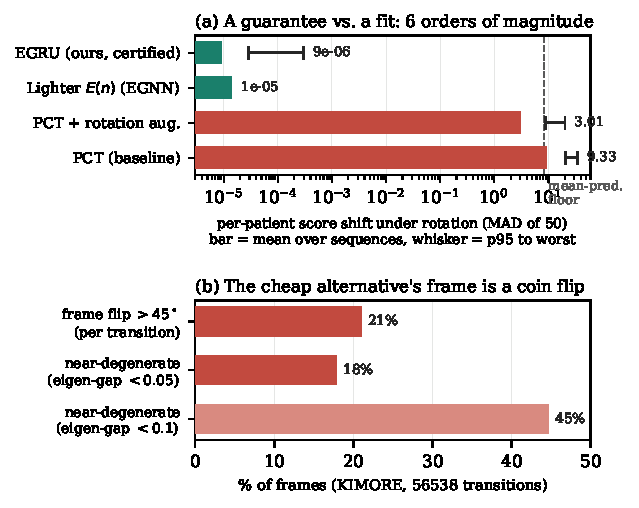
\includegraphics[width=\linewidth]{fig_guarantee}
  \caption{\textbf{The axis that separates the survivors.} (a)~Per-patient score shift under
  camera rotation (log scale). Bar is the mean over held-out sequences at the worst azimuth; whisker
  runs $95$th percentile to worst sequence. EGNN has no measured tail and carries no whisker.
  (b)~PCA frame instability: frame transitions flipping $>45^\circ$ ($21\%$), and frames within an
  eigen-gap of $0.05$ of degeneracy ($18\%$).}
  \label{fig:guarantee}
\end{figure}

\textbf{Canonicalization ties us offline --- and the difference is the guarantee.} The strongest
objection to an equivariant model is that a non-equivariant backbone fed a canonical frame reaches the
same place for less. It does, here: a per-frame PCA principal-axis frame feeding the transformer
(Canon-PCA$+$PCT, \cref{tab:pareto}) matches every offline axis --- clean $6.85$~MAD, $7.79$ at two dead
joints, and a viewpoint invariance empirically exact for arbitrary $SO(3)$, not merely the azimuth a
clinician sweeps (worst canonical-coordinate shift $3.7\times10^{-11}$ over $32$ random rotations).
This is the baseline's strong form: axes sign-disambiguated by a deterministic rule (each oriented so
its dominant joint projection is positive) and the frame forced right-handed, so the discrete $\pm$
ambiguity is resolved before any number below is measured.

The difference is not accuracy but \emph{conditioning}. Under a clean rotation the PCA frame is exactly
equivariant --- rotating the input sends the covariance to $RCR^{\!\top}$, whose eigenvectors are
exactly $RV$ --- and we measure that residual at $3\times10^{-6}$ degrees. But by
Davis--Kahan~\cite{daviskahan1970} an estimated eigenvector subspace moves by $O(\lVert E\rVert/\gamma)$
under a perturbation $E$ with eigen-gap $\gamma$, and a depth sensor supplies $E\neq0$ at every frame.
On KIMORE $\gamma$ is small far more often than not --- $18\%$ of frames within $0.05$ of degeneracy,
$45\%$ within $0.10$, a standing body being nearly axially symmetric --- so amplification is the
common case, not a corner. Injecting camera-frame noise at $2\%$ of body scale and comparing the frame
recovered at two camera poses, the residual rotation grows from $1.2^\circ$ where $\gamma>0.25$ to
$11.1^\circ$ where $\gamma<0.02$: a $9\times$ amplification, with $14.5\%$ of frames past $45^\circ$.

A better sign rule does not fix it. Replacing the dominant-joint convention with a third-moment rule
leaves the amplification intact ($12.1^\circ$, trimming only catastrophic flips to $11.1\%$), because a
sign rule resolves a \emph{discrete} ambiguity whereas degeneracy is a \emph{continuous} one. Temporal
smoothing is worse ($28.8^\circ$; $31.6\%$ past $45^\circ$): a frame locked onto the wrong branch
persists, and the frame becomes history-dependent, trading per-frame equivariance for lag. A learned point-estimate frame
inherits the same obstruction --- no canonicalizer is simultaneously exactly equivariant and continuous
where the configuration's stabilizer is non-trivial~\cite{kaba2023canon}. We report this at the frame
rather than the score: the frame measurement is model-free and binds any spectral canonicalizer,
whereas how much wobble survives to the output is corpus-dependent and secondary to whether the
mechanism exists. Our cut estimates \emph{no} frame: it is $SE(3)$-invariant for arbitrary weights by
construction (\cref{prop:invariance}), certified to roundoff over the full rotation group --- so the
\emph{same} certificate covers, without retraining, NTU~RGB+D Cross-View's displaced $45^\circ$
camera. A frame estimator offers neither the bound nor that transfer. We claim no accuracy win here
--- the tie is total; we claim a \emph{certified} worst case they structurally cannot offer, and
recommend the cheaper models where an off-distribution guarantee is not required.

\textbf{When the worst case is the deployment case.} A home device is set up by the patient and left
unattended: the camera sits wherever a phone stand or laptop lid lands, and the consumer depth sensor
is the component most likely to lose a joint. Neither cheaper alternative is safe against \emph{both}
conditions at once. Canon-PCA$+$PCT's viewpoint guarantee is only empirical --- \cref{fig:guarantee}b
puts the PCA frame within an eigen-gap of $0.05$ of degeneracy on $18\%$ of frames, where a flipped
frame is silent: no flag, just a wrong score. InvariantGRU's \emph{is} exact like ours, but its
named-joint features make it the most node-fail-fragile model measured: one frozen node drives it
from $6.31$ to $9.78$~MAD, through the floor (\cref{tab:nodefail}), the freeze mode a consumer sensor
exhibits routinely. Those are exactly the two conditions a home device cannot rule out in advance,
and EGRU is the only model measured provably safe against both --- not that the others are worse in a
fixed-rig clinic, but that neither offers a bound surviving unsupervised deployment.

\textbf{Second-corpus replication (REHAB24-6).} We replicate the structural story on REHAB24-6
(binary correct/incorrect repetitions; $1057$ reps, $10$ subjects; the
identical $0.66$M model as a BCE logit), an AUROC task over $3$ seeds and subject-disjoint CV
(\cref{tab:rehab246}). The accuracy tie holds --- EGRU $0.738\pm0.01$ versus the transformer
$0.707\pm0.02$ --- and, decisively, the viewpoint theorem transfers: under a $90^\circ$ camera rotation
EGRU's AUROC is \emph{unchanged} (logit drift $\le1.5\times10^{-4}$), while the transformer collapses to
chance ($0.52$). Node failure degrades both gracefully. The guarantee is thus not a KIMORE artifact ---
though at $10$ subjects this corpus replicates \emph{structural} properties, not accuracy: a certified
invariance either transfers exactly or it does not, and we draw no accuracy conclusion from it.

\begin{table}[t]\centering\small
\caption{REHAB24-6 second-corpus replication ($3$ seeds, subject-disjoint CV). AUROC@$90^\circ$ is the
same model evaluated under a $90^\circ$ camera rotation: EGRU is invariant by theorem (logit drift
$\le1.5\times10^{-4}$); the transformer falls to chance (drift $23.2$). Node-fail: AUROC lost over $8$
frozen nodes. The two models \emph{cross} between $2$ and $4$ frozen joints; full curve and fold-level
spread in the supplement.}
\label{tab:rehab246}
\resizebox{\columnwidth}{!}{%
\begin{tabular}{lccc}
\toprule
Model & AUROC & AUROC@$90^\circ$ & Node-fail lost \\
\midrule
\textbf{EGRU (ours)} & $\mathbf{0.738\pm0.01}$ & $\mathbf{0.738}$ & $+0.14$ \\
PCT (baseline)       & $0.707\pm0.02$ & $0.52\times$ & $\mathbf{+0.08}$ \\
\bottomrule
\end{tabular}}
\end{table}

\textbf{Per-family contribution of the cut.} Zeroing one family of \cref{eq:cut} at inference on the
deployed chiral model (dimension preserved, no retraining) resolves the mechanism to family
granularity (full table in the supplement). Two families carry accuracy --- the pairwise \emph{cosines}
($+1.83$~MAD to remove) and the learned \emph{triple products} ($+2.75$) --- and removing the cosines
is doubly harmful, inflating node-failure degradation the most ($+7.29$). The parity-odd families
\emph{split}: the learned triple products are relied upon while the fixed anatomical volumes are inert
($+0.19$), which reconciles rather than contradicts the chirality null --- that null is a \emph{retrain}
comparison (parity-even families substitute during training), whereas this is an \emph{inference}
ablation on a model trained \emph{with} the family.

\textbf{Two negative results, honestly --- each a mapped boundary of where structure pays.} (i) Native
consumption of irregular arrivals does not help on
KIMORE --- the fixed-grid baseline is better at every drop level under a hash-locked budget --- and a
spectral census~\cite{vanderplas2018lombscargle} predicts it: $97.7\%$ of \emph{positional} energy lies
below the resampling corner (though $70\%$ of \emph{velocity} energy lies above), so resampling
preserves pose geometry while low-passing the derivative band --- on KIMORE's healthy-form exercises
the discriminative signal is positional, so this acts as a denoiser; the boundary would move for
tremor-dominated tasks. The mechanism is real (a $5$~Hz
tremor is recovered at $r{=}1.000$ through $70\%$ drops where a resampled estimator decays to $0.785$),
so the claim is a scope boundary, not a defeat. (ii) Restoring chirality is principled but not rewarded
on healthy-form exercises with no chiral pathology --- the boundary at which a handedness prior stops
paying. Both are stated with the corpus properties that
would reward them (supplement).

% =====================================================================
\section{Deployment Analysis}\label{sec:edge}
We treat the guarantee as a systems property (\cref{tab:deploy}). \emph{Precision budget:} the
invariance floor climbs monotonically from fp64 to int8, and the int8 cliff is attributable
\emph{solely} to activation grid-rounding of the steerable channels --- weight quantization preserves
the theorem exactly (a quantized model is a different equivariant model) --- while the reported clinical
score still moves only $0.05$~MAD --- below the floor, $0.005$ of the between-subject SD, and one to two
orders of magnitude below the comparator MCID band established in \cref{sec:results}. \emph{Streaming:} because invariance lives in a
per-frame encoder and an invariant cut, the read-out converts to a strictly causal unidirectional form
with a running-mean pool that emits a first score $8.9$~ms after the first frame on an RTX-class GPU
(batch~1; $112$~fps, inside a $30$~fps budget) --- we report GPU latency as an upper bound on compute
and leave edge-SoC profiling to deployment --- reaching a usable prediction after $\sim\!55$ frames
(median), an honest time-to-first-\emph{reliable}-score for real-time use. The invariant read-out cut
is unchanged by the causal pooling, so \cref{prop:invariance} carries over verbatim; the cost is
$3.2$ points of NTU accuracy vs.\ the bidirectional model (NTU-60 X-View SOTA is $\sim\!92\%$; our
backbone is deliberately untuned --- we measure the streaming \emph{delta}, not absolute accuracy). A
canonicalization front-end would instead add a per-frame eigendecomposition to the hot path and
re-open the invariance question after quantization; here the guarantee is a fixed property of the
read-out and survives both int8 and causal streaming without re-certification. \emph{A real camera
move:} replaying one clip to a webcam from seven physical camera poses, our score moves $0.74$ of
fifty on average (worst $1.41$) against PCT's $2.16$ (worst $3.25$), a gap above $2\times$ under lag
and frame-rate perturbation. One subject, one exercise, and it bounds \emph{shift}, not accuracy ---
webcam skeletons are off-distribution for both --- and, as on NTU's three simultaneous cameras, ours
is not zero (supplement).

\begin{table}[t]\centering\small
\setlength{\tabcolsep}{4pt}
\caption{Deployment audit. Top: the \emph{full} equivariance precision budget of the deployed pooled
EGRU (INV floor = relative violation of the $160$-d parity-even projection; score shift in MAD of $50$).
fp16 is $3.2\times$ tighter than bf16 --- equivariance pays in mantissa bits, which bf16 trades for
exponent range --- and the int8 cliff is \emph{solely} activation grid-rounding (weight-only quant
preserves the theorem). Bottom: causal streaming vs.\ bidirectional read-out.}
\label{tab:deploy}
\resizebox{\columnwidth}{!}{%
\begin{tabular}{lccl}
\toprule
Arithmetic & INV floor & Score shift & Note \\
\midrule
fp64 & $5.75\times10^{-16}$ & $3.3\times10^{-14}$ & exact (theorem) \\
fp32 & $2.68\times10^{-7}$  & $8.9\times10^{-6}$  & $=$ main viewpoint \\
fp16 & $2.62\times10^{-3}$  & $0.024$             & $>$ bf16 \\
bf16 & $8.34\times10^{-3}$  & $0.195$             & mantissa cost \\
\midrule
int8, weights only     & $3.09\times10^{-7}$ & $1.2\times10^{-5}$ & theorem holds \\
int8, activations only & $3.38\times10^{-2}$ & $0.056$ & cliff (acts) \\
int8, weights$+$acts   & $\mathbf{3.40\times10^{-2}}$ & $\mathbf{0.051}$ & weight-quant.\ theorem-safe \\
\midrule
\multicolumn{4}{l}{Streaming: $8.9$~ms/frame ($112$~fps); read-out cut unchanged;} \\
\multicolumn{4}{l}{causal vs.\ bidir NTU X-View $79.8$ vs.\ $83.0$ ($-3.2$ pt).} \\
\bottomrule
\end{tabular}}
\end{table}

% =====================================================================
\section{Conclusion}\label{sec:conclusion}
On the metric the field reports, no architecture separates from another: on clean frontal KIMORE our
model, the baseline, and a hand-crafted-invariant GRU tie within a $0.33$~MAD nondeterminism floor --- the
metric is saturated. What separates them is off the frontal manifold. Our read-out is $SE(3)$-invariant by construction and
certified to machine roundoff, so relocating the camera moves a patient's score by $9\times10^{-6}$~MAD
for arbitrary weights, while a broken tracking node --- fatal to the hand-crafted model --- is absorbed
by the graph encoder; both properties replicate on a second corpus, and the guarantee survives to int8
and to causal streaming. We recommend the field report a mean-predictor floor and the per-sequence
degradation \emph{distribution} --- not only its mean, which on our own augmented baseline understates
the worst patient by nearly $7\times$ --- alongside aggregate error, and evaluate off the frontal
manifold: camera relocation and node failure are ordinary conditions of a home device, not adversarial
constructions.

\noindent\textbf{Code availability.} KIMORE~\cite{capecci2019kimore}, NTU~RGB+D and REHAB24-6 are
public. Our certificate, harnesses, benchmarks, and the script regenerating every number here from
banked artifacts will be released on acceptance; the URL is withheld for double-blind review.

% =====================================================================
\begin{thebibliography}{00}
\bibitem{capecci2019kimore} M.~Capecci et al., ``The KIMORE dataset: Kinematic assessment of movement and clinical scores for remote monitoring of physical rehabilitation,'' \textit{IEEE TNSRE}, vol.~27, no.~7, pp.~1436--1448, 2019.
\bibitem{pct2026} K.~Rafat, M.~I.~Hossain, M.~M.~L.~Elahi, S.~Momen, F.~Rahman, N.~Mohammed, and S.~Rahman, ``A point cloud transformer for remote monitoring and automated assessment of physical rehabilitation exercises,'' \textit{IEEE J. Biomed. Health Inform.}, 2026, accepted; arXiv:2606.30309.
\bibitem{karlov2024} M.~Karlov, A.~Abedi, and S.~S.~Khan, ``Rehabilitation exercise quality assessment through supervised contrastive learning with hard and soft negatives,'' \textit{Med. Biol. Eng. Comput.}, 2024.
\bibitem{abedi2023} A.~Abedi, M.~Malmirian, and S.~S.~Khan, ``Cross-modal video to body-joints augmentation for rehabilitation exercise quality assessment,'' arXiv:2306.09546, 2023.
\bibitem{kuang2026} Z.~Kuang et al., ``Dual-stream STGCN with motion-aware grouping for rehabilitation action quality assessment,'' \textit{Sensors}, vol.~26, no.~1, p.~287, 2026.
\bibitem{rehabpile2026} A.~Ismail-Fawaz et al., ``Rehab-Pile: A cross-subject rehabilitation benchmark aggregating KIMORE, UI-PRMD and IRDS,'' arXiv:2507.21018, IEEE FG 2026.
\bibitem{vakanski2018uiprmd} A.~Vakanski et al., ``A data set of human body movements for physical rehabilitation exercises (UI-PRMD),'' \textit{Data}, vol.~3, no.~1, p.~2, 2018.
\bibitem{yan2018stgcn} S.~Yan, Y.~Xiong, and D.~Lin, ``Spatial temporal graph convolutional networks for skeleton-based action recognition,'' in \textit{Proc. AAAI}, 2018.
\bibitem{cohen2016gconv} T.~S.~Cohen and M.~Welling, ``Group equivariant convolutional networks,'' in \textit{Proc. ICML}, 2016.
\bibitem{thomas2018tfn} N.~Thomas et al., ``Tensor field networks: Rotation- and translation-equivariant neural networks for 3D point clouds,'' arXiv:1802.08219, 2018.
\bibitem{fuchs2020se3transformer} F.~B.~Fuchs et al., ``SE(3)-Transformers: 3D roto-translation equivariant attention networks,'' in \textit{Proc. NeurIPS}, 2020.
\bibitem{geiger2022e3nn} M.~Geiger and T.~Smidt, ``e3nn: Euclidean neural networks,'' arXiv:2207.09453, 2022.
\bibitem{satorras2021egnn} V.~G.~Satorras, E.~Hoogeboom, and M.~Welling, ``E(n) equivariant graph neural networks,'' in \textit{Proc. ICML}, 2021.
\bibitem{deng2021vectorneurons} C.~Deng et al., ``Vector neurons: A general framework for SO(3)-equivariant networks,'' in \textit{Proc. ICCV}, 2021.
\bibitem{puny2022frameaveraging} O.~Puny et al., ``Frame averaging for invariant and equivariant network design,'' in \textit{Proc. ICLR}, 2022.
\bibitem{daviskahan1970} C.~Davis and W.~M.~Kahan, ``The rotation of eigenvectors by a perturbation. III,'' \textit{SIAM J. Numer. Anal.}, vol.~7, no.~1, pp.~1--46, 1970.
\bibitem{kaba2023canon} S.-O.~Kaba et al., ``Equivariance with learned canonicalization functions,'' in \textit{Proc. ICML}, 2023.
\bibitem{chen2018neuralode} R.~T.~Q.~Chen et al., ``Neural ordinary differential equations,'' in \textit{Proc. NeurIPS}, 2018.
\bibitem{rubanova2019odernn} Y.~Rubanova, R.~T.~Q.~Chen, and D.~Duvenaud, ``Latent ODEs for irregularly-sampled time series,'' in \textit{Proc. NeurIPS}, 2019.
\bibitem{kidger2020neuralcde} P.~Kidger et al., ``Neural controlled differential equations for irregular time series,'' in \textit{Proc. NeurIPS}, 2020.
\bibitem{che2018grud} Z.~Che et al., ``Recurrent neural networks for multivariate time series with missing values,'' \textit{Sci. Rep.}, vol.~8, p.~6085, 2018.
\bibitem{dormand1980prince} J.~R.~Dormand and P.~J.~Prince, ``A family of embedded Runge--Kutta formulae,'' \textit{J. Comput. Appl. Math.}, vol.~6, no.~1, pp.~19--26, 1980.
\bibitem{vanderplas2018lombscargle} J.~T.~VanderPlas, ``Understanding the Lomb--Scargle periodogram,'' \textit{ApJS}, vol.~236, no.~1, p.~16, 2018.
\end{thebibliography}

\end{document}
